\documentclass{article} % Tipo de documento
\usepackage[utf8]{inputenc} % Permite el uso de caracteres del Español
\usepackage[T1]{fontenc}
\usepackage{graphicx}
\usepackage{amsmath}
\usepackage{wrapfig}
\usepackage{enumerate}
\usepackage[top=1in, bottom=1.25in, left=1.1in, right=1.1in]{geometry}

% Carátula del Artículo

\title{Reporte de Actividad 1}

\author{José Gabriel Navarro Islas}

\date{23 de Enero, 2018}

\begin{document}

\maketitle 

\section{Introducción}
En el presente reporte se habla acerca de la Atmósfera Terrestre y varias de sus características y propiedades. Este reporte corresponde a la primera actividad del curso de Física Computacional I, para la Lic. en Física de la Universidad de Sonora. \\

Este reporte abarca varios temas, uno de ellos es la composición de la atmósfera, es decir que constituye a la atmósfera. La estructura de la atmósfera es otro de los temas tocados, en donde se habla acerca de las cinco principales capas de nuestra atmósfera además de otras capas. También se mencionan las propiedades físicas de ella, abarcando la presión, espesor, temperatura, velocidad del sonido, masa y densidad. Otro aspecto importante son las propiedades ópticas de la atmósfera, ya que la radiación solar es absorbida y reflejada por la atmósfera, lo cual causa distintos fenómemos ópticos, como lo son la dispersión, la absorción, la emisión y el índice de refracción. Por ultimo se habla acerca de la circulación de la atmósfera, en donde se abarca el movimiento del aire en ella.

\section{Composición}

\begin{wrapfigure}{r}{0.3\textwidth}
    \centering
    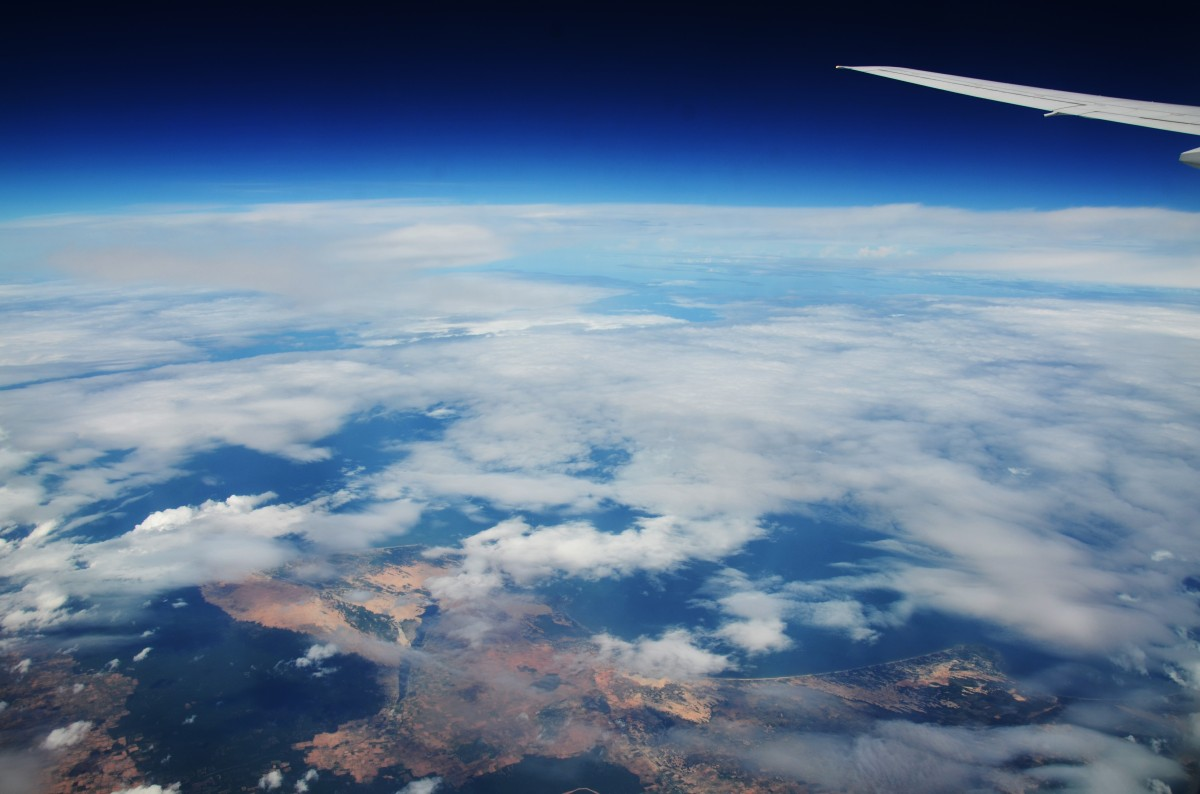
\includegraphics[width=0.35\textwidth]{atm1.jpg}
    \caption{Toma de la atmósfera terrestre}
\end{wrapfigure}

Los tres constituyentes principales del aire terrestre, y por tanto de la atmósfera terrestre son el nitrógeno, el oxigeno y el argón. El vapor de agua conforma el 0.25\% de la masa de la atmósfera, la concentración de esta puede variar de hasta 10 ppm por volumen en las partes frías de la atmósfera hasta 5\% por volumen en áreas calientes. \\

Los otros gases que componen la atmósfera, entre ellos los gases de efecto invernadero, se encuentran el dióxido de carbono, el metano, el oxido nitroso y el ozono. El aire filtrado contiene varios compuestos químicos, los cuales pueden ser tanto naturales, (polvo de composiciones orgánicas y minerales, polén, esporas y ceniza volcánica) como industriales, (cloro, flúor y mercurio en vapor).

\section{Estructura de la atmósfera}

En general la presión del aire y la densidad decrece con la altitud de la atmósfera. Sin embargo la temperatura se comporta de una manera mas complicada con el aumento de la altitud, dependiendo de la altitud, la temperatura se mantiene casi constante, lo cual es de mucha ayuda al clasificar las capas de la atmósfera. Entonces se pueden clasificar como: \\\\\\\\

\begin{figure}[h]
    \centering
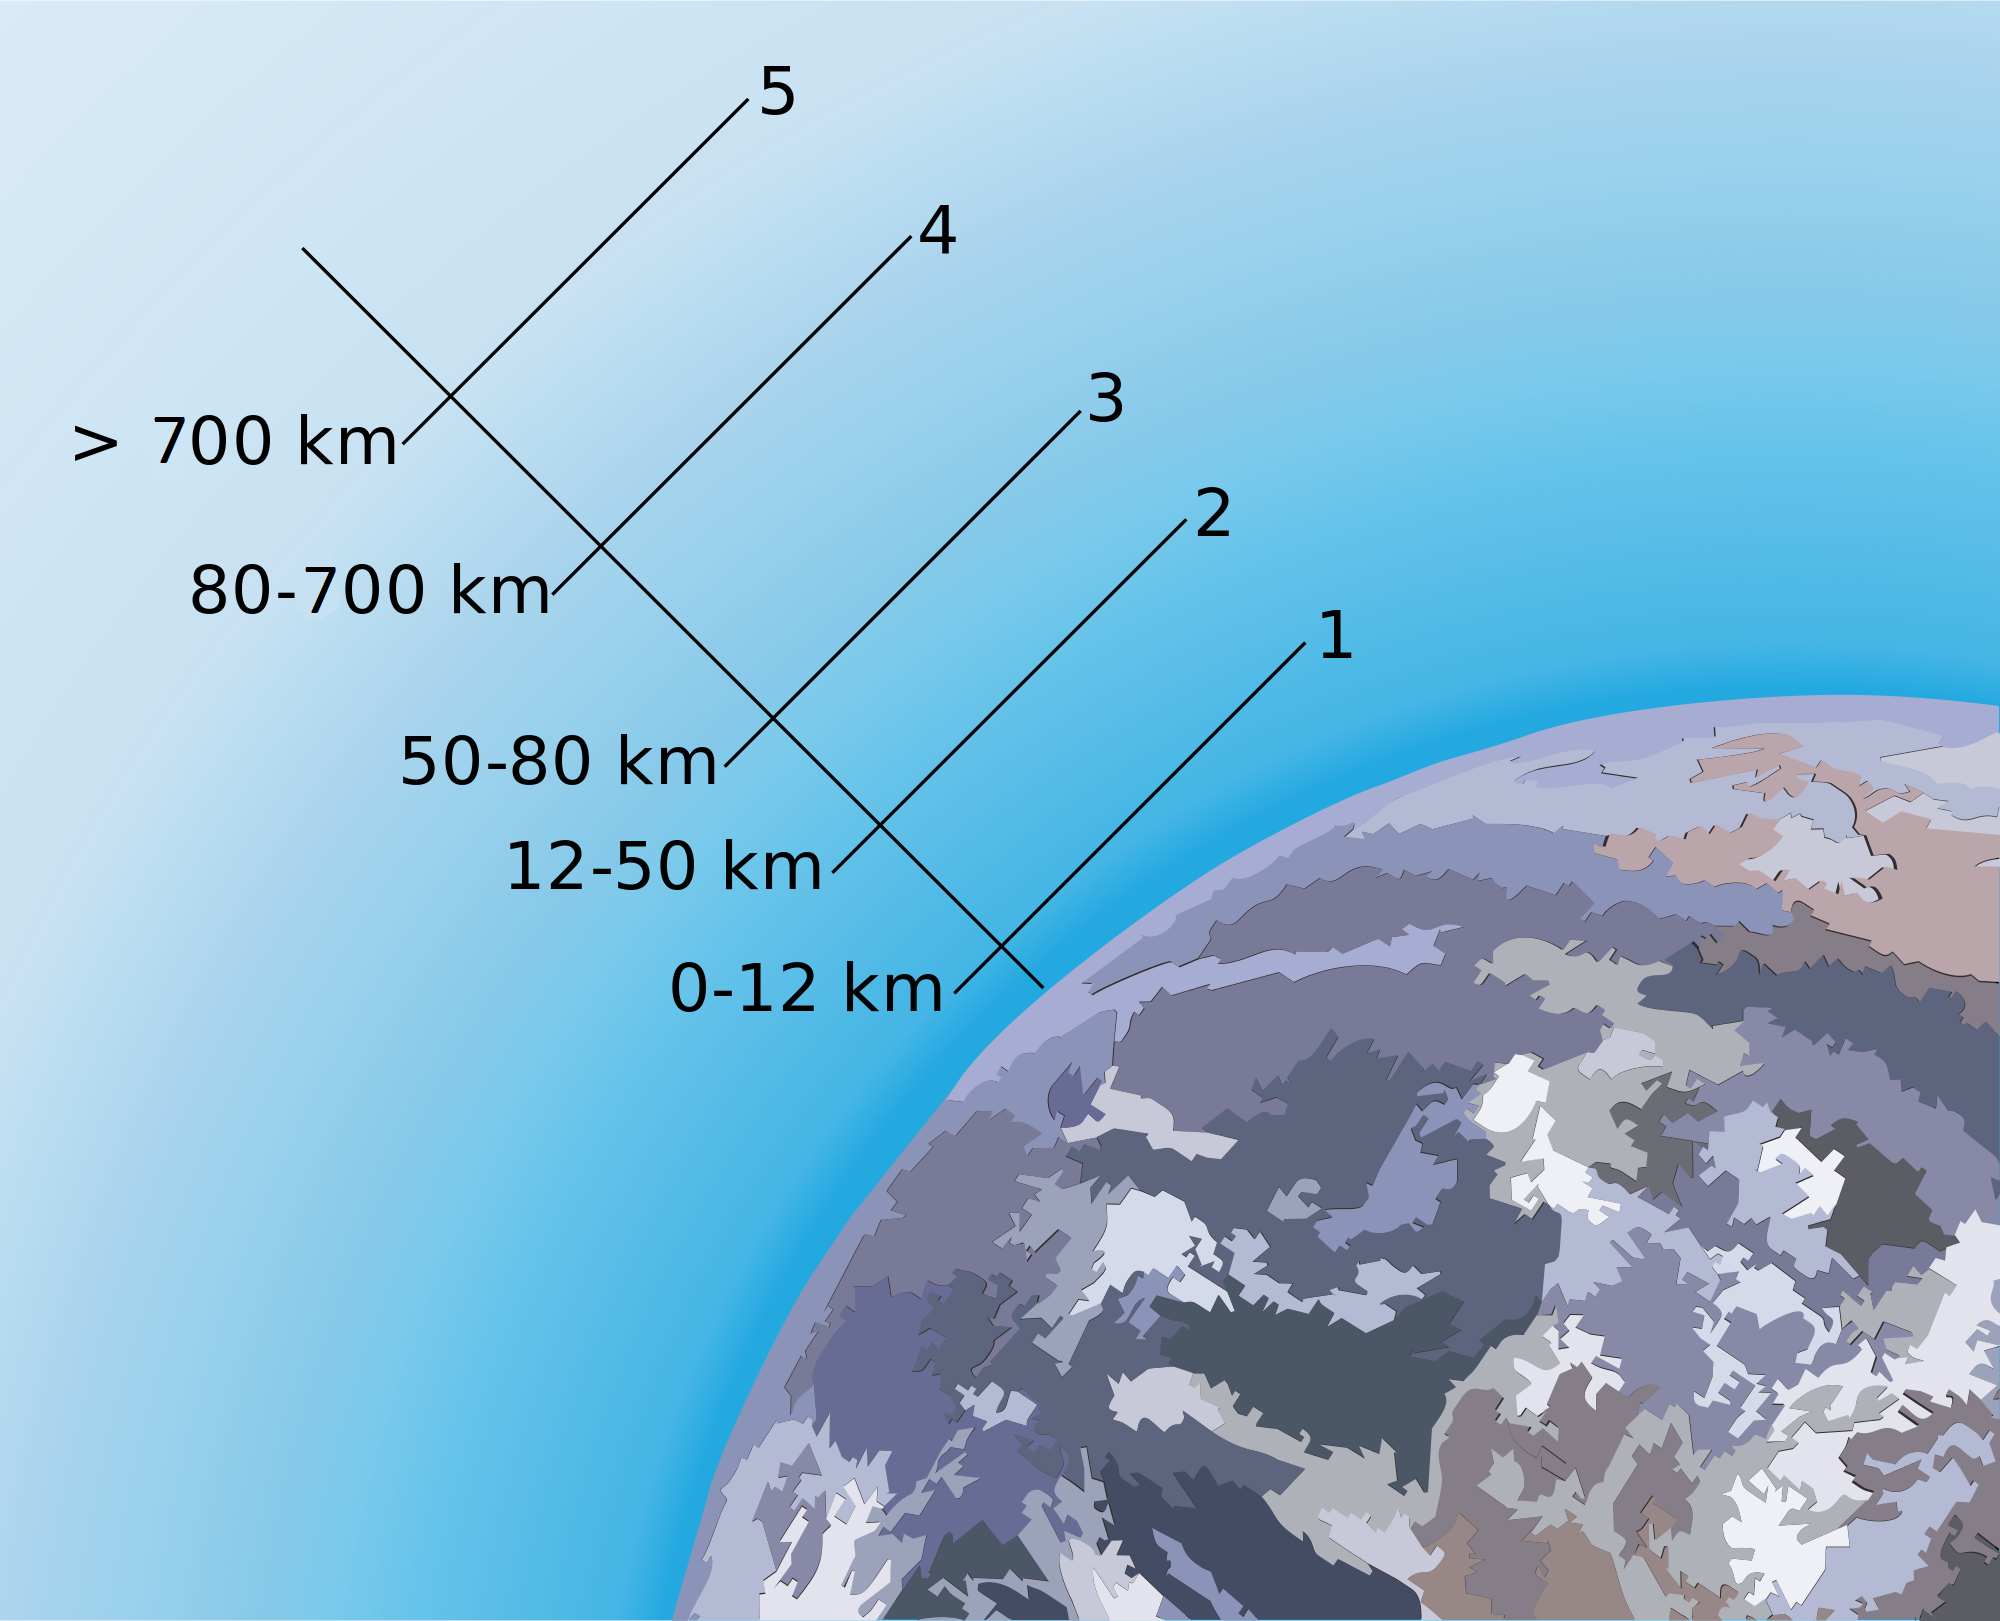
\includegraphics[width=3in]{atm2.png}
\end{figure}

\begin{enumerate}
    \centering
    \item Troposfera: De 0 a 12 km
    \item Estratosfera: De 12 a 50 km
    \item Mesosfera: 50 a 80 km
    \item Termosfera: De 80 a 700 km
    \item Exosfera: De 700 a 10,000 km
\end{enumerate}


\subsection{Capas Principales}
\subsubsection{Exosfera}
La exosfera es la capa más lejana de la atmosfera terrestre. Esta compuesta principalmente de bajas densidades de hidrogeno, helio y varias moléculas pesadas incluyendo el nitrógeno, oxígeno y dióxido de carbono. Como esta no se comporta como gas, las partículas pueden escapar hacia el espacio, las cuales pueden migrar a la magnetosfera.\\

Debido a que esta tan alejada de la Tierra, no puede ser posible que existan fenómenos meteorológicos. Sin embargo, las auroras a veces se encuentran en la parte baja de la exosfera. Además esta capa contiene la mayoría de los satélites que orbitan a la Tierra.

\begin{wrapfigure}{r}{0.25\textwidth}
    \centering
    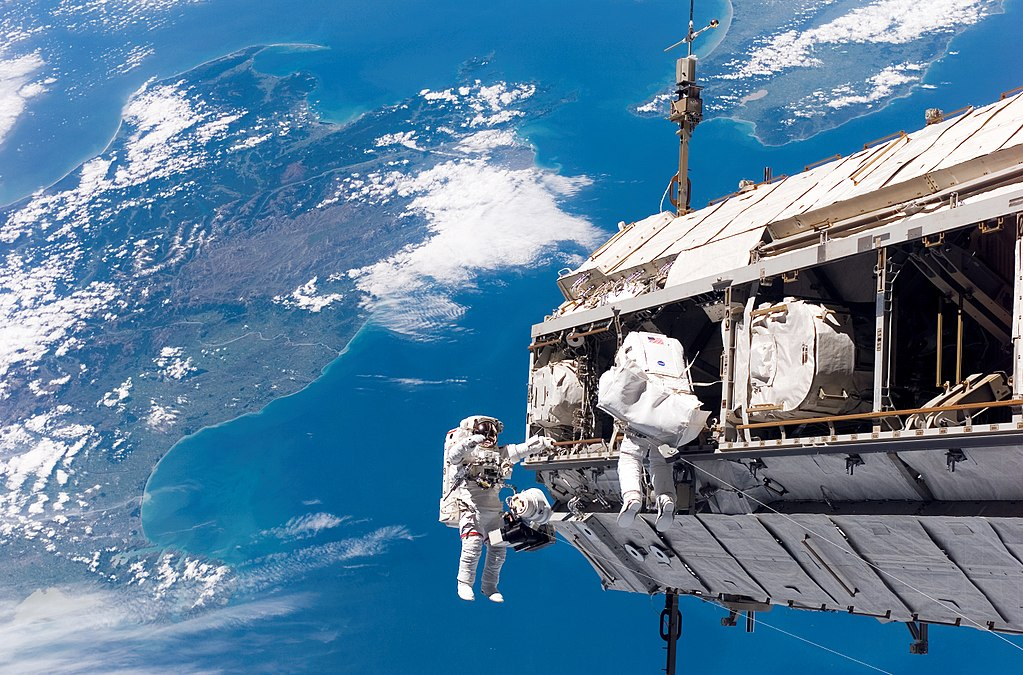
\includegraphics[width=0.3\textwidth]{estacion.jpg}
\end{wrapfigure}

\subsubsection{Termosfera}
La termosfera es la segunda capa mas alejada de la Tierra y contiene la ionosfera.  La temperatura de ella incrementa gradualmente con la altura y al contrario de la estratosfera, donde la inversión térmica de la temperatura es debido a la absorción de la radiación de ozono, la inversión en la termosfera es debido a la baja densidad de las moléculas. Su temperatura puede llegar hasta temperaturas de 1500 $^{\circ}$C, sin embargo, a pesar de que existe una gran proporción de moléculas con altas energías, si un humano la tocara, no se sentiría tan caliente, ya que la densidad de las moléculas es demasiado baja como para conducir suficiente energía hacia la piel.\\

Esta capa esta libre de nubes y de vapor de agua , pero las auroras pueden verse ocasionalmente en la termosfera. La Estación Espacial Internacional orbita en esta capa, entre los 350 y 420 km.

\subsubsection{Mesosfera}
La mesosfera es la tercera capa mas lejana de la Tierra, ocupando la región entre la estratosfera y debajo de la termosfera. Las temperaturas bajan cuando aumenta la altitud, por lo cual es el lugar mas helado de la Tierra, su temperatura media esta entre los -85 $^{\circ}$C. \\

El aire es tan helado que el vapor de agua puede ser sublimada a nubes mesosféricas. Estas nubes son las más altas en la atmósfera y pueden ser observadas por el ojo humano si la luz del sol las refleja después de la puesta de sol. La mesosfera es demasiada alta como para ser accesible para aviones jet y globos, y demasiado abajo para permitir orbitar, es por eso que solo los cohetes sonda acceden a esta capa.

\subsubsection{Estratosfera}
La estratosfera es la segunda capa mas baja de la atmósfera terrestre. Esta arriba de la troposfera y separada de ella por la tropopausa.  La presión atmosférica es acerca de 1/1000 de la presión al nivel del mar. Contiene la capa de ozono, que es la parte de la atmósfera de la Tierra que contiene gran cantidad de gases.  El aumento en temperatura es causado por la absorción de la radiación ultravioleta. A pesar de que la temperatura en la tropopausa es alrededor de -60 $^{\circ}$C, en la parte superior de la estratosfera es 0 $^{\circ}$C.\\

La temperatura de la estratosfera crea condiciones atmosféricas muy estables, así que la estratosfera no puede crear la turbulencia de aire que es predominante en la troposfera. Es por esa misma razón que esta capa es libre de nubes y cualquier otro tipo de clima. Esta es la capa mas alta que puede alcanzar un avión o jet.


\subsubsection{Troposfera}
La troposfera es la capa mas baja de la atmosfera terrestre. Se extiende desde la superficie de la Tierra, donde su altura depende del lugar, varia entre los 9 km hasta los 17 km en el ecuador. Aunque si ocurren variaciones, la temperatura usualmente declina con el aumento de altitud, ya que esta capa esta siendo calentada por la transferencia de energía de la superficie. Cabe mencionar que esta capa contiene el 80\% de la masa de la atmosfera, y es mas densa que todas las demás capas ya que esta siendo comprimida por estas mismas.\\

Casi todo el vapor de agua o humedad esta contenida en la troposfera, por lo cual es la capa en donde casi todos los eventos relacionados al clima suceden. La aviación mas convencional toma lugar en esta capa y es la única capa que puede ser accesada por aviones de hélice. 

\subsection{Otras capas}
Las 5 capas principales de la atmósfera se clasifican por temperatura, pero existen otras capas que pueden ser clasificadas con otras propiedades: 
\begin{itemize}
    \item La capa de ozono esta contenida en la estratosfera. La concentración de ozono es alrededor de 2 a 8 ppm, que es mucho mas alta que en la capa mas baja de la atmósfera. Esta localizada principalmente en la porción mas baja de la estratosfera.
    \item La ionosfera es una región de la atmósfera que esta ionizada por radiación solar. Es la responsable de las auroras. Durante el día se estira de 50 a 1000 km, e incluye a la mesosfera, termosfera, y partes de la exosfera. 
    \item La homósfera y heterosfera están definidas si los gases atmosféricos están bien mezclados. La homósfera incluye a la troposfera, estratosfera, mesosfera y la parte más baja de la termosfera, donde la composición química de la atmósfera no depende del peso molecular. Arriba de esta se encuentra la heterosfera que incluye la exosfera y la mayoría de la termosfera. Aquí la composición química depende de la altitud, esto es porque la distancia que las partículas se pueden mover sin colisionarse con otras es grande comparado con el tamaño de los movimientos que causan el mezclarse. La parte mas alta de la heterosfera esta compuesta casi de puro hidrogeno.
    \item La capa límite planetaria es la parte de la troposfera que esta mas cerca a la superficie terrestre y es directamente afectada por ella. Durante el día esta capa usualmente esta bien mezclada, y su rango de altura es desde los 100 metros en noches claras y calmadas, hasta 3000 metros o mas en regiones secas.
\end{itemize}

\section{Propiedades Físicas}

\subsection{Presión y Espesor}
La presión atmosférica promedio a nivel del mar es de 101325 pascales. Este valor es usualmente referido como 1 atm. La masa atmosférica total es de $5.148 * 10^8  kg$, 2.5\% menos de lo que se infería   de la presión promedio del nivel del mar.\\

Sin embargo, la atmósfera es mejor modelada con una ecuación para para cada capa, en donde se toma en cuenta las condiciones, como lo son la temperatura, la composición molecular, la radiación solar y la gravedad. En resumen, la masa de la atmósfera puede distribuirse como sigue: 50\% esta debajo de 5.5 km, 90\% esta debajo de los 16 km, y el 99.99997\% esta debajo de los 100 km.

\subsection{Temperatura y velocidad del sonido}
Como ya se menciono anteriormente, la temperatura decrece con el aumento de la altitud empezando desde el nivel del mar, pero variaciones de esto empiezan a partir de los 11 km, donde la temperatura se estabiliza durante una gran distancia vertical. En la estratosfera empezando por arriba de los 20 km, la temperatura aumenta con la altura, debido al calentamiento dentro de la capa de ozono causado por la captura de radiación ultravioleta del Sol.\\

Debido a que la velocidad del sonido depende solo de la temperatura y no de la presión y densidad del gas o medio en el que se propaga, la velocidad del sonido en la atmósfera toma la forma del perfil complicado de la temperatura, y no refleja cambios altitudinales en densidad o presión.


\subsection{Masa y Densidad}
La densidad del aire a nivel del mar es de 1.2 $kg/m^3$. La densidad no es medida directamente, pero es calculada por las medidas de temperatura, presión y humedad usando la ecuación del estado del aire. La densidad atmosférica decrece cuando la altitud incrementa. La masa de la atmósfera  es aproximadamente de 5 cuatrillones de toneladas.

\begin{center}
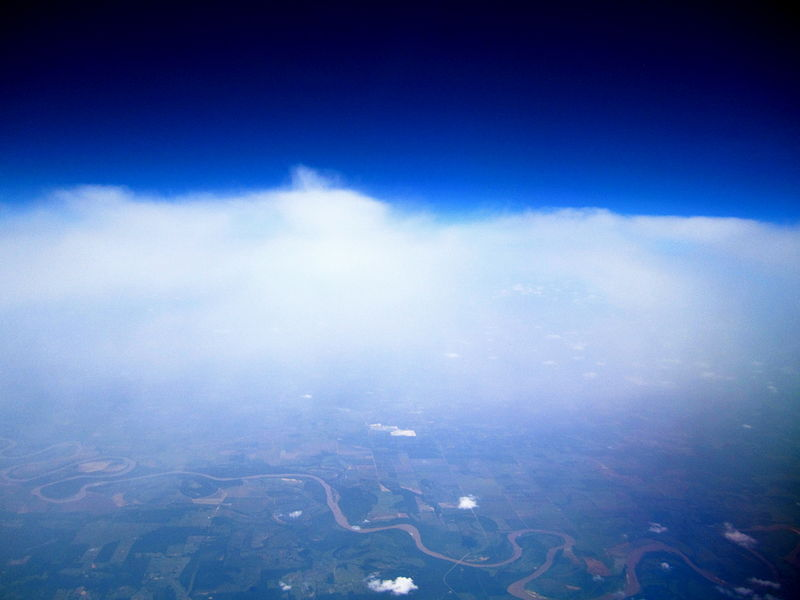
\includegraphics[scale=0.3]{atm3.jpg}
\\Según el Centro Nacional de Investigación Atmosférica la masa total de la atmósfera es 5.1480 $* 10^{18}$ con un rango anual por vapor de agua entre 1.2 y 1.5 $* 10 ^{15}$.
\end{center}

\section{Propiedades Ópticas}
La radiación solar es la energía que recibe la Tierra debido al Sol, parte de la radiación que entra es absorbida o reflejada por la atmósfera. Esto hace que la atmósfera tenga distintas propiedades ópticas, las cuales se discuten a continuación.

\subsection{Dispersión}
Cuando la luz pasa a través de la atmósfera terrestre, fotones interactúan con ella mediante la dispersión. Si la luz no interactúa con la atmósfera, se le llama entonces radiación directa y es lo que se ve cuando se mira directamente al Sol. Radiación indirecta es la luz que ha sido dispersada en la atmósfera. Un ejemplo de esto es el fenómeno llamado Dispersión de Rayleigh, que explica como longitudes de onda mas cortas se dispersan más fácil que las rojas, y es por lo que nuestro cielo se ve azul y las puestas de sol son rojas.

\subsection{Absorción}
Diferentes moléculas absorben distintas longitudes de onda de radiación. Por ejemplo, el agua absorbe muchas de las ondas mayores a 700 nm. Cuando una molécula absorbe un fotón, incrementa la energía de la molécula. Esto calienta a la atmósfera, pero la atmósfera también se enfría emitiendo radiación.\\

La combinación del espectro de absorción de los gases en la atmósfera deja “ventanas” de opacidad baja, permitiendo la transmisión de ciertas bandas de luz.

\subsection{Emisión}
La emisión es lo opuesto a la absorción, esta sucede cuando un objeto emite radiación. Los objetos tienden a emitir cantidades de ondas de radiación dependiendo de las curvas de emisión de su cuerpo negro, por lo tanto, objetos mas calientes tienden a emitir mas radiación, con longitudes de onda mas cortas. Si un objeto esta helado, este emite menos radiación, pero con ondas de mayor longitud.\\

Debido a su temperatura, la atmósfera emite radiación infrarroja Durante noches claras en la superficie, una persona puede notar que se enfría más rápido que en una noche nublada. Esto se debe a que las nubes son absorbedores fuertes de radiación infrarroja. El efecto invernadero esta relacionado con estos dos fenómenos, la absorción y la emisión.

\subsection{Índice de refracción}
El índice de refracción del aire esta cerca, pero no es mayor a 1. Variaciones en el índice de refracción pueden llevar a la curvatura de los rayos de luz en caminos largos de vista. El índice de refracción depende de la temperatura, haciendo que los efectos de la refracción aumenten cuando la temperatura es grande. Un ejemplo de estos son los espejismos.

\section{Circulación}
La circulación atmosférica es el movimiento del aire a gran escala alrededor de la troposfera, y los medios por los cuales el calor es distribuido alrededor de la Tierra. La circulación varia cada año, pero la estructura básica se mantiene constante por la rotación de la Tierra y la diferencia en la radiación solar entre el ecuador y los polos.

\begin{figure}[h!]
  \centering
    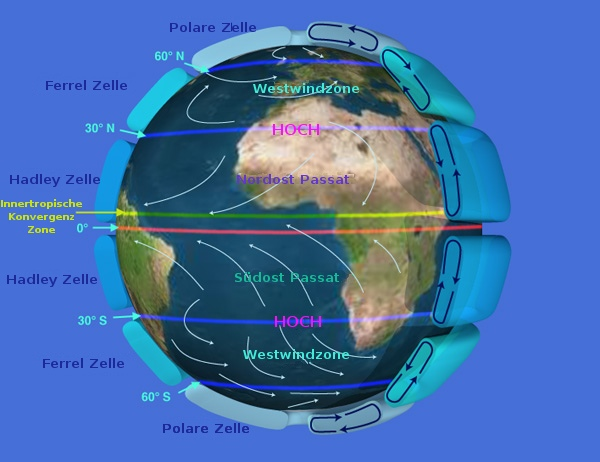
\includegraphics[width=0.5\textwidth]{circulacion.jpg}
\end{figure}

\section{Apéndice}

\textbf {1. ¿Qué fue lo que más te llamó la atención de esta actividad?}\\\\
El entorno y sintaxis que utiliza LaTeX, es como programar un texto, lo cual me parece algo muy curioso. Anteriormente lo había utilizado en otras clases, pero no lo suficiente como para descubrir otras funciones interesantes. \\

\noindent\textbf {2. ¿Qué fue lo que se te hizo menos interesante?}\\\\
El tema del que trataba la sintesis se me hizo un poco extenso, es muy interesante, pero pienso que podría ser mas corto. \\

\noindent\textbf {3. ¿Qué cambios harías para mejorar esta actividad?}\\\\
Proporcionar un manual de LaTeX con las funciones basicas para hacer listas, colocar imagenes de distintas maneras, y otras funciones para así encontrar directamente la función y paquete que se debe usar. Muchas veces encontraba la sintaxis en la que se debía escribir una función en LaTeX pero no mostraba el paquete correspondiente y no podía usarla. \\\\

\noindent\textbf {4. ¿Cuál es tu primera impresión de uso de LATEX?}\\\\
Es un lenguaje interesante que nos permite tener mas herramientas para insertar funciones y ecuaciones de una manera mas fácil y ágil, además de que al escribir el código, se muestra el resultado directamente, lo cual ayuda mucho. \\\\

\noindent\textbf {5. ¿El tiempo sugerido para esta actividad fue suficiente?} \\\\
Si, el tiempo fue suficiente para realizar la practica. \\

\noindent\textbf {6. ¿Encontraste algún documento o recurso en línea útil que quisieras compartir con los demás?} \\\\
Si, encontre una pagína que habla acerca de varias librerias de LaTeX y su uso, de esta pagina pude encontrar varias funciones que utilice en el reporte, como lo fue el colocar imagenes alineadas y dentro del texto, listas enumeradas, entre otras cosas la página es: https://es.sharelatex.com/learn/

\section {Bibliografía}

\begin{itemize}
    \item Portillo, G. (2017, Mayo 8) Capas de la atmósfera. Recuperado de: www.meteorologiaenred.com/capas-atmosfera.html
    \item Atmosphere of Earth. (2018, Enero 24). Recuperado de: en.wikipedia.org/wiki/Atmosphere\_of\_Earth
    \item Circulación atmosférica. (2017, Diciembre 13). Recuperado de:
es.wikipedia.org/wiki/Circulación\_atmosférica \\
\end{itemize}

Imagenes utilizadas: 
\begin{itemize}
    \item Imagen 1: Fecha: 08/09/17, (pxhere), pxhere.com/en/photo/1417102
    \item Imagen 2: Fecha: 26/10/14, (Wikimedia), commons.wikimedia.org/wiki/File:Atmosphere\_structure\_numbered.svg
    \item Imagen 3: Fecha:12/12/06, (NASA) en.wikipedia.org/wiki/Space\_station\#/media/File:STS-116\_spacewalk\_1.jpg
        \item Imagen 4: Fecha:17/12/10, (Wikimedia) https://commons.wikimedia.org/wiki/File:Atmosphere\_(6044045761).jpg
    \item Imagen 5: Fecha: 23/05/08, (Wikimedia), https://commons.wikimedia.org/wiki/File:Earth\_Global\_Circulation\-DE.jpg

\end{itemize}

\end{document}